\section{Simpl DSL Toolkit}


\subsection{Note}

In general, the following text assumes that the artifacts and tasks
(such as procedure lifting) are explained in the main part of the
paper and that this section only needs to provide information about
how a given task was solved using the tool.


\subsection{Introduction}

Simpl is a toolkit mainly targeted at implementing domain-specific
languages (DSLs) in an enterprise setting. In particular, the goal
is to be able to embed Simpl into a larger system. Freudenthal \cite{enterprise-dsl}
analyzes the technical requirements for embeddable DSL tools and reviews
existing DSL tools based on these requirements.

In order to be embeddable, a DSL toolkit should consist of two separate
parts. One, {}``non-visual'' part contains the core of the DSL implementation:
parser, program checker, code generator, etc. that can be embedded
into a larger system. The other, {}``visual'' part contains (possibly
integrated) environment for editing and managing DSL programs. Secondly,
the non-visual part of the DSL implementation should not make any
assumptions on how the system is implemented. In particular, the non-visual
part must not have dependencies to visual part and must not assume
that the DSL implementation is a top-level program or function in
the system.

Simpl is designed to follow these non-functional requirements while
providing maximal usability. The current design philosophy of Simpl
is to reuse existing tools to minimize the amount of new tools and
programming languages the developer must learn. For example, instead
of developing a new language for expressing program transformations,
Simpl relies on Scala programming language. In addition to Scala,
Simpl builds on ANTLR parser generator \cite{antlr}, Eclipse IDE
platform, and IDE Meta-Tooling Platform (IMP) \cite{imp}. The main
rationale for selecting these particular tools is that they are mature,
have good quality and are distributed under open source licences.
Tools that make up the non-visual part of the DSL implementation have
few dependencies and can be easily embedded (and can coexist with
other DSL tools). From the integration point of view, the main restricting
choice is using Eclipse as the IDE platform -- if the DSL user wants
to use IDE developed via Simpl, she must install Eclipse. In this
case, we chose the most popular platform.

%
\begin{figure}[!h]
\begin{centering}
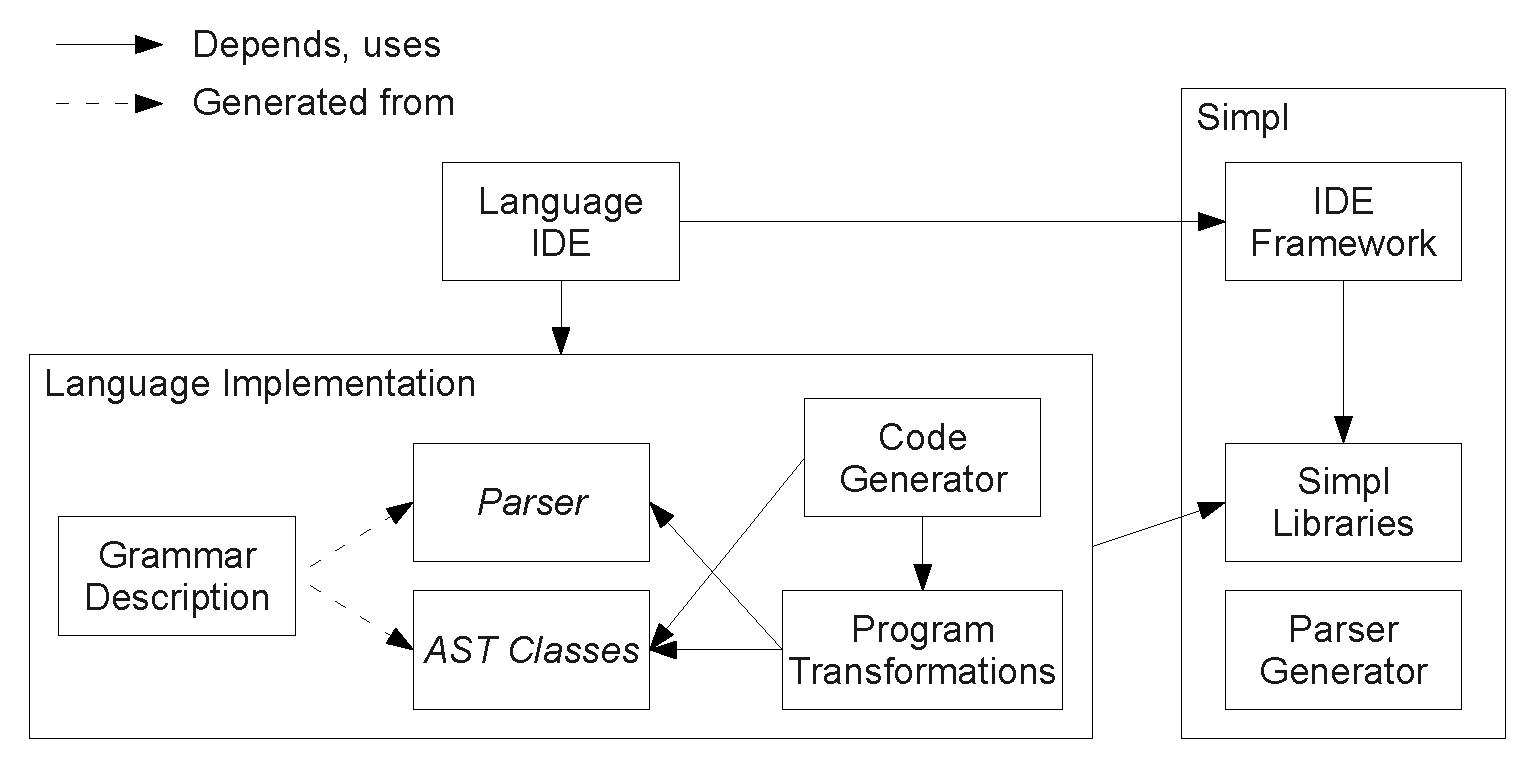
\includegraphics[width=0.7\columnwidth]{simpl/architecture.pdf}
\par\end{centering}

\caption{\label{fig:architecture}Architecture of a DSL implemented with Simpl.
Components with captions in italic are automatically generated.}

\end{figure}


Figure~\ref{fig:architecture} shows the main components of a DSL
implementation created with Simpl. The first part is the non-visual
language implementation that can be embedded into a bigger system.
Development of a new DSL starts with grammar description that specifies
both the context-free grammar of the DSL and the classes for representing
the abstract syntax tree (AST) of a DSL program. The Simpl parser
generator takes the grammar description as input and produces a parser
and the AST classes. The (optional) program transformation component
takes as input an AST and checks or transforms it. The code generator
converts the preprocessed AST to text. The second part of the DSL
implementation is the language IDE. It builds on Simpl IDE framework
and the non-visual part of the language implementation.


\subsection{Scanning and Parsing}

In Simpl, the grammar description is used to generate both the parser
and Scala case classes that are used to express the abstract syntax
tree (AST) of the DSL program. By default, the AST class and attribute
names are derived from rule names. The developer can add annotations
in the context-free grammar to modify the generated AST classes. As
an example, Figure \ref{fig:case-statement} shows set of rules for
parsing the Oberon0 \emph{CASE} statement. The identifiers before
the equals signs name the attributes in the case class that is used
for representing the AST. Figure \ref{fig:Automatically-generated-AST}
shows the Scala case classes that were generated from the example
rules. The attribute types are automatically derived from types of
called rules. If an attribute refers to rule(s) that can be called
multiple times, then the type of the attribute will be a list. For
example \emph{clauses} attribute in the \emph{CaseStatement} class
is typed as list because there can be more than one clause in one
case statement. Using the same attribute name several times in a rule
is allowed if the rule calls assigned to this attribute have compatible
type.

%
\begin{figure}[!h]
{\small }
\begin{lstlisting}[basicstyle={\footnotesize\ttfamily}]
CaseStatement:
    "CASE" expr=CompExpr "OF"
        clauses=CaseClause ("|" clauses=CaseClause)*
        ("ELSE" elseClause=StatementSequence)?
    "END";

CaseClause:
    items=CaseConstant ("," items=CaseConstant)* ":"
        stmt=StatementSequence;

CaseConstant: begin=SimpleExpr (".." end=SimpleExpr)?;
\end{lstlisting}
{\small \par}

\caption{\label{fig:case-statement}Grammar rules for parsing the Oberon0 \emph{CASE}
statement.}

\end{figure}


%
\begin{figure}[!h]
{\small }
\begin{lstlisting}[basicstyle={\footnotesize\ttfamily}]
case class CaseStatement(
    var expr: Expression, 
    var clauses: List[CaseClause], 
    var elseClause: StatementSequence) extends Statement

case class CaseClause(
    var items: List[CaseConstant],
    var stmt: StatementSequence)

case class CaseConstant(
    var begin: Expression, 
    var end: Expression)
\end{lstlisting}
{\small \par}

\caption{\label{fig:Automatically-generated-AST}AST classes for expressing
the Oberon0 \emph{CASE }statement.}

\end{figure}


Simpl allows modifying the generated AST classes using return expressions.
Return expressions can specify return type of a rule and/or a Scala
expression that is used to compute the actual AST node returned by
the rule. In the Oberon0 implementation, return expressions were used
to make the AST more regular and uniform. Figure \ref{fig:Using-return-expressions}
shows two examples. The first rule ensures that the use of parentheses
does not introduce additional wrapping of the AST nodes. The second
rule makes all the unary expressions use a common AST class \emph{Unary(operation,~expression)}
so that they can be uniformly treated in the processing code. 

%
\begin{figure}[!h]
{\small }
\begin{lstlisting}[basicstyle={\footnotesize\ttfamily}]
ParenExpr returns Expression {expr}: "(" expr=CompExpr ")";

NotExpr
    returns Expression {Unary(UnaryOp.Not, expr)}
    : "~" expr=Factor;
\end{lstlisting}
{\small \par}

\caption{\label{fig:Using-return-expressions}Example rules using return expressions.
Rule \emph{ParenExpr} does not wrap the inner AST node. Rule \emph{NotExpr}
returns manually created AST class.}

\end{figure}






In addition to return expressions, Simpl supports adding attributes
and methods to AST classes. For example, the code for parsing identifiers
is shown in Figure \ref{fig:Adding-properties}. This code modifies
the normally generated \emph{Id} class to add attributes for storing
references to definition of this identifier, pre-calculated constant
values if this identifier evaluates to constant expression, and information
whether the identifier is a by-ref procedure parameter. These attributes
are filled out and used during name, type checking and code generation.

%
\begin{figure}[!h]
{\small }
\begin{lstlisting}[basicstyle={\footnotesize\ttfamily}]
terminal Id {
    // What does this identifier point to?
    var ref: Id = null
    // If this is constant, then what is its value?
    var constVal: Option[Int] = None
    // Used for "VAR" parameters.
    var byRef: Boolean = false
    def isByRef = byRef || ((ref ne null) && (ref.byRef))
} : ('a'..'z'|'A'..'Z') ('a'..'z'|'A'..'Z'|'0'..'9')*;
\end{lstlisting}
{\small \par}

\caption{\label{fig:Adding-properties}Rule for parsing identifiers. The generated
class \emph{Id} is amended by adding properties and methods to it.}

\end{figure}



\subsection{Name Analysis}

Simpl has no direct support, therefore the name analysis for the Oberon0
language was written in Scala. The implementation is quite straightforward:
it walks through the AST and for each identifier fills out its \emph{ref}
attribute (points from identifier, such as variable reference, to
declaration of this identifier. See also Figure \ref{fig:Adding-properties}).
During the walk, we maintained an environment: a mapping from identifier
names to declarations.






\subsection{Type Checking}

Like name analysis, type checking was implemented in Scala. Since
name analysis was run before type checking, there was no need to use
environments (mappings from names to types). Instead, the type checker
first attached type information to all the declared identifiers (variables,
constants, procedure parameters). It then propagated the type information
to all expressions and procedure calls and checked the types of operation
arguments and procedure call parameters.  According to task definition,
checking for negative array sizes was also part of type checking,
therefore the type checker computed values of all constant expressions
and stored the values in the AST.




\subsection{Source-to-Source Transformation}

In order to simplify C code generation, the Simpl implementation transformed
Oberon0 programs to simplify Oberon0 language constructs that have
no direct equivalent in the C programming language. The first transformation
lifted nested procedures to top level. The second transformation replaced
\emph{CASE} statements with sequence of \emph{IF} statements.


\subsubsection{\label{sub:Procedure-Lifting}Procedure Lifting}

Procedure lifting used links created during the name analysis step
and performed in-place modifications of the AST. The task was accomplished
in three steps. First step consisted of scanning the AST and locating
all the nested procedures. Figure \ref{fig:Program-before-lifting}
shows an example Oberon0 program with the inner procedure highlighted.
In the second step, all the nested procedures were lifted to top level.
The new name was formed by concatenating names of outer and inner
procedures. If the concatenation did not produce unique name, a number
was added to the name. Figure \ref{fig:Program-during-lifting} shows
the results of this step with the lifted procedure highlighted. Finally,
the AST was scanned and all identifiers that referenced the lifted
procedures were renamed to reflect the new names. Figure \ref{fig:Program-after-lifting}
shows the end result with the renamed identifier highlighted.

%
\begin{figure}[!h]
\begin{tabular}{>{\centering}p{0.33\textwidth}>{\centering}p{0.33\textwidth}>{\centering}p{0.33\textwidth}}
{\scriptsize }
\begin{lstlisting}[basicstyle={\footnotesize\ttfamily},escapechar={\%},showlines=true]
PROGRAM Foo;
    PROCEDURE Bar;
        %\texttt{\textbf{PROCEDURE Baz;}}%
        %\texttt{\textbf{END Baz;}}%
    BEGIN
        Baz
    END Bar;
BEGIN
    Bar
END Foo.
 
\end{lstlisting}
{\scriptsize \par}

\subfloat[\label{fig:Program-before-lifting}]{} & {\scriptsize }
\begin{lstlisting}[basicstyle={\footnotesize\ttfamily},escapechar={\%}]
PROGRAM Foo;
    %\texttt{\textbf{PROCEDURE BarBaz;}}%
    %\texttt{\textbf{END BarBaz;}}%
 
    PROCEDURE Bar;
    BEGIN
        Baz
    END Bar;
BEGIN
    Bar
END Foo.
\end{lstlisting}
{\scriptsize \par}

\subfloat[\label{fig:Program-during-lifting}]{} & {\scriptsize }
\begin{lstlisting}[basicstyle={\footnotesize\ttfamily},escapechar={\%}]
PROGRAM Foo;
    PROCEDURE BarBaz;
    END BarBaz;
 
    PROCEDURE Bar;
    BEGIN
        %\texttt{\textbf{BarBaz}}%
    END Bar;
BEGIN
    Bar
END Foo.
\end{lstlisting}
{\scriptsize \par}

\subfloat[\label{fig:Program-after-lifting}]{}\tabularnewline
\end{tabular}

\caption{Three stages of procedure lifting: locating nested procedures (a),
lifting the procedures (b), and renaming the procedure references
(c).}

\end{figure}



\subsubsection{\label{sub:Simplifying-CASE-Statements}Simplifying \emph{CASE} Statements}

The Oberon0 \emph{CASE} statement is more powerful than \emph{switch}
statement in C programming language as it has support for ranges.
In order to simplify code generation, we transformed Oberon0 \emph{CASE}
statements to series of \emph{IF}-\emph{ELSE }statements (see Figure
\ref{fig:CASE-statement} for an example transformation). We generate
new variable for storing the \emph{CASE} condition. Because the results
of \emph{CASE} simplification will go straight to C code generation,
we can optimize by not making the generated identifier \emph{gen\_1}
a legal Oberon0 identifier. This way we do not have to ensure that
it does not clash with any identifiers in this scope.

%
\begin{figure}[!h]
\begin{tabular}{>{\centering}p{0.35\textwidth}>{\centering}p{0.55\textwidth}}
{\footnotesize }
\begin{lstlisting}[basicstyle={\footnotesize\ttfamily},showlines=true]
CASE foo + bar OF
      1 : Write(1)
    | 3..4 : Write(34)
ELSE
    Write(-1)
END;
 
 
  
 
\end{lstlisting}
{\footnotesize \par}

\subfloat[\label{fig:case-before}]{} & {\footnotesize }
\begin{lstlisting}[basicstyle={\footnotesize\ttfamily}]
VAR gen_1: INTEGER;
...
gen_1 := foo + bar;
IF gen_1 = 1 THEN
    Write(1)
ELSE IF gen_1 >= 3 AND gen_1 <= 4 THEN
    Write(34)
ELSE
    Write(-1)
END;
\end{lstlisting}
{\footnotesize \par}

\subfloat[\label{fig:case-after}]{}\tabularnewline
\end{tabular}

\caption{\emph{\label{fig:CASE-statement}Oberon0 CASE} statement before (a)
and after transformation (b).}

\end{figure}



\subsection{Code Generation}

When implementing C code generation, we decided to decouple translating
Oberon0 language constructs to C from outputting properly formatted
C code. This allowed us to concisely express the transformation between
Oberon0 AST to C AST without concerning the pretty-printing of C code.
First, we created Scala case classes for expressing abstract syntax
of the C language. Next, Oberon0 AST was transformed to C AST. Because
the more complicated Oberon0 constructs were previously simplified
(see the previous subsection), the translation was quite straightforward.
In the last step, the C AST was transformed to string using pretty-printing
library included in Simpl.

Figure \ref{fig:code-generation} illustrates the code generation
process with an example procedure for calculating factorial. Since
Oberon0 has no functions, the result is returned in a \emph{VAR} parameter.
Whereas AST of the Oberon0 \emph{FOR} statement (see Figure \ref{fig:code-generation}b)
corresponds to Oberon0 syntax, the translated \emph{for} statement
(see Figure \ref{fig:code-generation}c) corresponds to C syntax (initialization
and increment are statements, guard is an arbitrary expression). During
the translation, all the identifiers are prefixed with underscore
to prevent clashes with existing keywords.

%
\begin{figure}[!h]
\begin{tabular}{>{\raggedright}p{0.48\textwidth}>{\centering}p{0.48\textwidth}}

\begin{lstlisting}[basicstyle={\footnotesize\ttfamily},escapechar={\%}]
PROCEDURE Fact(
    n: INTEGER;
    VAR Res: INTEGER);
  VAR i: INTEGER;
BEGIN
  Res := 1;
  %\texttt{\textbf{FOR i := 1 TO n DO}}%
    %\texttt{\textbf{Res := Res * i;}}%
  %\texttt{\textbf{END}}%
END Fact;
\end{lstlisting}


(a) Oberon0 source before code generation. & 
\begin{lstlisting}[basicstyle={\footnotesize\ttfamily}]
ForStatement(
 Id(i),
 NumberLit(1),
 Id(n),
 null,
 StatementSequence(
  List(
   Assignment(
   Id(Res),
   Binary(*,Id(Res),Id(i))))))
\end{lstlisting}


(b) Oberon0 AST corrensponding to the highlighted \emph{FOR} statement.\tabularnewline

\begin{lstlisting}[basicstyle={\footnotesize\ttfamily}]
For(
 Assign(
  Id(_i,false),
  NumberLit(1)),
 Binary(
  <=,
  Id(_i,false),
  Id(_n,false)),
 Inc(_i,NumberLit(1)),
 Sequence(
  List(
   Assign(
    Id(_Res,true),
    Binary(
     *,
     Id(_Res,true),
     Id(_i,false))))))
\end{lstlisting}


(c) \emph{FOR} statement translated to AST representing a C program. & 
\begin{lstlisting}[basicstyle={\footnotesize\ttfamily},escapechar={\%},showlines=true]
void _Fact(int _n,int *_Res) {
  int _i;
  (*_Res) = 1;
  %\texttt{\textbf{for (\_i = 1; \_i <= \_n; \_i += 1) \{}}%
    %\texttt{\textbf{({*}\_Res) = ({*}\_Res) {*} \_i;}}%
  %\texttt{\textbf{\}}}%
}
 
 
 
 
 
 
 
 
 
 
\end{lstlisting}


(d) C source generated from the function in sub-figure (a). The highlighted
\emph{for} statement corresponds to AST from sub-figure (c).\tabularnewline
\end{tabular}

\caption{\label{fig:code-generation}Code generation example: translating the
procedure from Oberon0 to C.}

\end{figure}



\subsection{Artifacts}

The Oberon0 implementation is composed of five different artifacts
(A1, A2a, A2b, A3, A4). Each artifact either adds additional constructs
to the language or adds additional features, such as type checking,
procedure lifting or code generation. Table \ref{tab:loc-statistics}
shows code sizes for different artifacts and tasks. Code size is measured
in lines of code; empty lines and comments were not counted. For counting
lines of code, we used program \emph{cloc}%
\footnote{see \url{http://cloc.sourceforge.net/}%
} that was extended with support for Simpl grammar files. In the table,
each row represents size of a particular component:
\begin{itemize}
\item Parse -- Simpl grammar file and any additional Scala code (such as
custom classes for expressing binary operators and checks that numerical
constants fit into 32 bits);
\item Name -- code for name analysis;
\item Type -- code for type checking and and constant inlining%
\footnote{Constant inlining is used to check for negative array sizes.%
};
\item Lift -- code for lifting nested procedures to top level;
\item Gen -- code generator, including simplification of \emph{CASE} statements,
transforming Oberon0 AST to C AST, and pretty-printing C AST;
\item Pretty -- pretty-printing of Oberon0 code;
\item Other -- other supporting code, such as error handling, main functions,
etc.
\end{itemize}
%
\begin{table}[!h]
\caption{\label{tab:loc-statistics}Code sizes for different artifacts and
components. Sizes are expressed as non-blank, non-comment lines of
code.}


\noindent \centering{}\begin{tabular}{|c|r|r|r|r|r|r|r|r|}
\hline 
Artifact/Component & Parse & Name & Type & Lift & Gen & Pretty & Other & \textbf{Total}\tabularnewline
\hline
\hline 
A1 & 193 & 181 &  &  &  &  & 44 & \textbf{418}\tabularnewline
\hline 
A2a & 38 & 135 &  &  &  &  & 16 & \textbf{189}\tabularnewline
\hline 
A2b &  &  & 301 &  &  &  & 17 & \textbf{318}\tabularnewline
\hline 
A3 &  &  & 92 &  &  &  & 17 & \textbf{109}\tabularnewline
\hline 
A4 & 48 & 44 & 89 & 72 & 463 & 198 & 39 & \textbf{953}\tabularnewline
\hline 
\textbf{Total} & \textbf{279} & \textbf{360} & \textbf{482} & \textbf{72} & \textbf{463} & \textbf{198} & \textbf{133} & \textbf{1987}\tabularnewline
\hline
\end{tabular}
\end{table}


Except for A1, the artifacts are not self-contained in the terms of
code. The artifacts reuse grammar files and Scala code. Figure \ref{fig:artifact-dependencies}
shows the dependency graph between artifacts. The grammar files are
reused by using include directive. For example, L3 grammar includes
L2 grammar and overwrites production rules for declarations (by adding
procedure declaration) and statements (by adding procedure calls).
Services written in Scala, such as name analysis and type checking,
were extended using inheritance. In general, the extension consisted
in overriding \emph{processStatement}, \emph{processExpr} etc. methods
and adding new case clauses to process additional kinds of statements
or expressions.

%
\begin{figure}[!h]
\noindent \begin{centering}
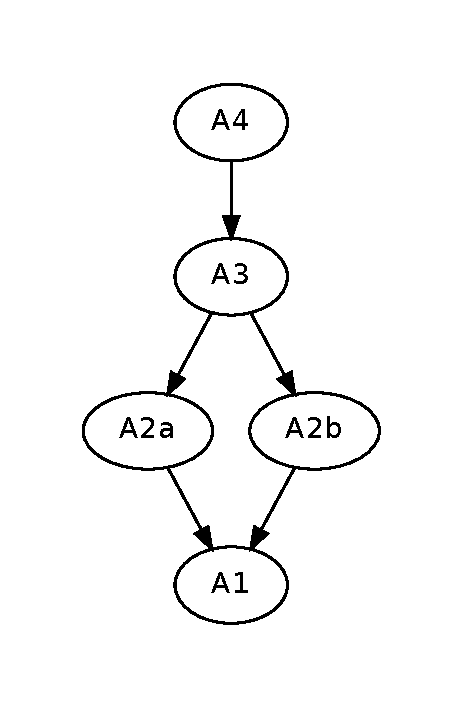
\includegraphics[scale=0.5]{simpl/artifacts.pdf}
\par\end{centering}

\caption{\label{fig:artifact-dependencies}Dependencies between artifacts in
the Oberon0 implementation.}

\end{figure}


In addition to artifacts mandated in the challenge, we used Simpl
to implement basic IDE for the Oberon0 language (see Figure \ref{fig:Screenshot-of-Oberon0}
for example screenshot). The IDE provided syntax highlighting, error
highlighting, outline view, hyperlinking, code folding, and occurrence
marking. The total code size for the IDE module was 106 lines, some
of which was filler. Most of the Oberon0-related functionality was
encapsulated in a 33-line class that contained IDE services. The IDE
code was based on the existing code checker (artifact A4) and did
not involve references to Eclipse APIs. 

%
\begin{figure}[!h]
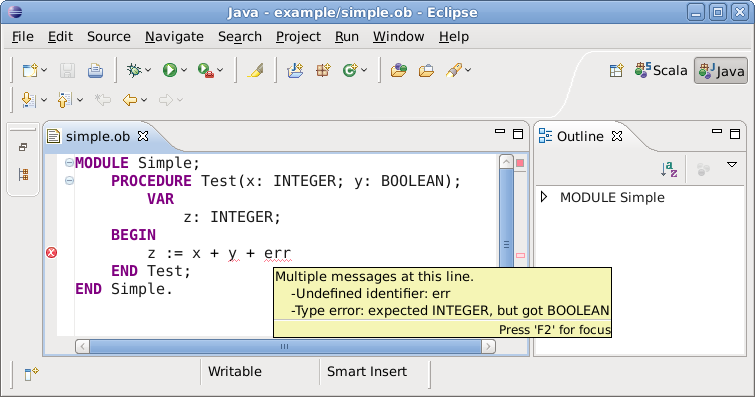
\includegraphics[width=12cm]{simpl/ide-screenshot.png}

\caption{\label{fig:Screenshot-of-Oberon0}Screenshot of Oberon0 IDE}

\end{figure}





\subsection{Observations}

First, it should be noted that Simpl is not directly targeted at creating
full-featured implementations of typical programming languages. Currently
the focus is on domain-specific languages and quite simple code generators.
Therefore, Simpl provided direct support for a subset of all the tasks
contained in this challenge. In particular, we used Simpl to create
a parser and class model for expressing AST of Oberon0 programs, and
for pretty-printing the AST. Although not included in challenge task,
we also used Simpl to create an IDE for the Oberon0 language.

Simpl currently uses ANTLR as a parser backend and therefore inherits
the use of \emph{LL(k)} parsing algorithm. The \emph{LL(k)} algorithm
has trouble expressing left-recursive grammar rules and thus parsing
left-associative operators. This limitation means that operator precedence
must be encoded in grammar rules%
\footnote{In this challenge the grammar was already specified in this form.%
} and it also results in cumbersome AST. The cumbersome AST can be
worked around by using return expressions that shape the AST nodes
returned by the grammar rules. In the future, we plan to use parser
backend that does not have this restriction.

Simpl grammar system is not specifically targeted at implementing
modular grammars. It only supports simple inclusion mechanism with
the ability to overwrite rules in the included grammars. In the challenge
exercise, this introduced minor code duplication. For example, in
order to introduce new kind of statement, one has to repeat the \emph{Statement}
rule with all the other preexisting statements. Overall, for the modularity
features were adequate for the current situation where there were
language levels with increasing complexity and each following level
added new constructs to the language. However, if the task were to
require highly modular grammars, then the current modularity features
likely would not have sufficed.


\subsection{Conclusions}

In general, implementing the challenge with Simpl was a straightforward
exercise. The grammar description was legible and the automatically
generated AST classes worked well with processing code written in
Scala. Simpl does not have support for implementing program checkers
and program tranformation, therefore these functions were written
in straight Scala. In addition to required tasks, we implemented an
IDE for Oberon0. The IDE was based on challenge code and required
minimal amount of effort to create.

